\documentclass[mathserif,18pt,xcolor=table,c]{beamer}

% Load Beamer Style Theme
% TAMU Based
\usepackage{tamu_beamer}
% \usepackage[skip=0pt]{caption}

% Specifiy the location of images to be used
\graphicspath{{figures/}}

% ------------------------------------------------------------
% ------------------------------------------------------------
% ------------------------------------------------------------
% ----------------TITLE PAGE----------------------------------
% ------------------------------------------------------------
% ------------------------------------------------------------
% ------------------------------------------------------------
% Document Title Page
\title{Surface wave supporting structures in the terahertz and optical frequency domains}
% \subtitle{Preliminary Exam}
\author[Hasan Tahir Abbas]{Hasan Tahir Abbas\\~\\{\small {Supervised by: Dr. Robert D. Nevels}}}
\institute{Department of Electrical  \& Computer Engineering\\ \mbox{} \\ \pgfuseimage{tamuecenbig}}
\date[Summer 2017]{\today}
% ------------------------------------------------------------
% ------------------------------------------------------------
% ------------------------------------------------------------
% ------------------------------------------------------------
% ------------------------------------------------------------
% ------------------------------------------------------------
% ------------------------------------------------------------
% ------------------------------------------------------------
% ------------------------------------------------------------
% ------------------------------------------------------------
% ------------------------------------------------------------
% ------------------------------------------------------------
% ------------------------------------------------------------
% ------------------------------------------------------------
\begin{document}

% Reduce space around equations and subequations
\preto\subequations{\ifhmode\unskip\fi}
\AtBeginEnvironment{subequations}{\ifhmode\unskip\fi}
\AtBeginEnvironment{equation}{\ifhmode\unskip\fi}

% Draw Boxes in the footer with pertinent info
\tikzstyle{block} = [rectangle, draw, rounded corners, shade, top color=white, text width=5em,
bottom color=blue!50!black!20, draw=blue!40!black!60, very thick, text centered, minimum height=4em]
\tikzstyle{line} = [draw, -latex']
\tikzstyle{cloud} = [draw, ellipse,top color=white, bottom color=red!20, node distance=2cm, minimum height=2em]

% Tick Style
\beamertemplateballitem
% \beamertemplatetransparentcoveredhigh

\frame{\titlepage}


% Add TAMU logo on each slide in the north-east side
% Shifted to be right at the edge
%
% NOTE: Will have to compile twice
%
\addtobeamertemplate{frametitle}{}{%
\begin{tikzpicture}[remember picture,overlay]
  \node[anchor=north east,yshift=7pt,xshift=2pt] at (current page.north east) {
\includegraphics[height=.7cm]{ecen}};
\end{tikzpicture}}
% ------------------------------------------------------------
% ------------------------------------------------------------
% ------------------------------------------------------------
% ------------------------------------------------------------
% ------------------------------------------------------------
% ------------------------------------------------------------
% ------------------------------------------------------------
% ------------------------------------------------------------
% ------------------------------------------------------------
% ------------------------------------------------------------
% ------------------------------------------------------------
% ------------------------------------------------------------
% ------------------------------------------------------------
% ------------------------------------------------------------
\section{Outline}
\begin{frame}
  \frametitle{Outline}
  \begin{outline}[itemize]
    \1 Plasmonics Overview
    \1 Background
    \1 Theory and Methods
      \2 Sommerfeld Integral analysis
      \2 Dispersion relation
      \2 Surface Integral equation
    \1 Results
    \1 Conclusions
  \end{outline}
\end{frame}
% ------------------------------------------------------------
% ------------------------------------------------------------
% ------------------------------------------------------------
% ------------------------------------------------------------
% ------------------------------------------------------------
% ------------------------------------------------------------
% ------------------------------------------------------------
% ------------------------------------------------------------
% ------------------------------------------------------------
% ------------------------------------------------------------
% ------------------------------------------------------------
% ------------------------------------------------------------
% ------------------------------------------------------------
\section{Overview}
% ------------------------------------------------------------
% ------------------------------------------------------------
\begin{frame}
  \frametitle{Plasmonics Overview}
  % ----------------------------------------------------------
  \begin{columns} % align columns
    \begin{column}{.5\textwidth}
      \begin{outline}[itemize]
        \1 Interaction of electromagnetic (EM) waves with free electrons
        \1 Subwavelength localization of EM fields
        \1 Plasma frequency
          \2 Metals - Optical frequency
          \2 Semiconductors - Terahertz
        \1 Low efficiency
      \end{outline}
    \end{column}
    \begin{column}{.5\textwidth}
      % Use this to preserve fonts from Inkspace
      \begin{figure}
        \hspace*{-1cm}
        % \vspace*{-2cm}
        \def\svgwidth{1.2\linewidth}
        \input{figures/scale.pdf_tex}
        \caption{Communication Technologies at various frequencies}
      \end{figure}
      \end{column}%
    \end{columns}
  \end{frame}
% ------------------------------------------------------------
% ------------------------------------------------------------
% ------------------------------------------------------------
% ------------------------------------------------------------
% ------------------------------------------------------------
% ------------------------------------------------------------
% ------------------------------------------------------------
% ------------------------------------------------------------
% ------------------------------------------------------------
% ------------------------------------------------------------
% ------------------------------------------------------------
\section{Overview}
% ------------------------------------------------------------
% ------------------------------------------------------------
\begin{frame}
  \frametitle{Plasmonics Overview}
  % \framesubtitle{Optical frequency}
  % ----------------------------------------------------------
  \begin{columns} % align columns
    \begin{column}{.5\textwidth}
      \begin{outline}[itemize]
        \1 Metal-dielectric interface
        \1 Surface plasmon polaritons (SPPs)
        \end{outline}
        \begin{equation} \nonumber
          \Re \left[ \E_{\text{metal}}(\O)\right] < 0
        \end{equation}
        \begin{outline}[itemize]
        \1 Plasma frequency
          \2 Metals - Optical frequency
          \2 Semiconductors - Terahertz
        \1 Low efficiency
      \end{outline}
    \end{column}
    \begin{column}{.5\textwidth}
      % Use this to preserve fonts from Inkspace
      \begin{figure}[b!]
        \hspace*{-1cm} \vspace*{0.5cm}
        \def\svgwidth{1.15\linewidth}
        \input{figures/spp.pdf_tex}
        \label{fig:spp}
      \end{figure}
      \end{column}%
    \end{columns}
  \end{frame}
% ------------------------------------------------------------
% ------------------------------------------------------------
% ------------------------------------------------------------
% ------------------------------------------------------------
% ------------------------------------------------------------
% ------------------------------------------------------------
% ------------------------------------------------------------
\section{Background}
% ------------------------------------------------------------
% ------------------------------------------------------------
% ------------------------------------------------------------
% ------------------------------------------------------------
% ------------------------------------------------------------
% ------------------------------------------------------------
% ------------------------------------------------------------
% ------------------------------------------------------------
% ------------------------------------------------------------
% ------------------------------------------------------------
% ------------------------------------------------------------
% ------------------------------------------------------------
% ------------------------------------------------------------
% ------------------------------------------------------------
\section{Background}
\begin{frame}
  \frametitle{Background}
  \framesubtitle{Surface Plasmons}

  \begin{columns} % align columns
    \begin{column}{.5\textwidth}
      \begin{minipage}[T][.1\textheight][c]{\linewidth}
        \begin{outline}[itemize]
          \1 Metal-dielectric interface
          \1 Surface plasmon polaritons (SPPs)
          \1 Slow surface waves
            \2 Wavelength
            \2 Semiconductors - Terahertz
          \1 Low efficiency
        \end{outline}
        \begin{itemize}
          \item Metal-dielectric interface
        \end{itemize}
        \begin{itemize}
          \item Slow surface waves
          \item Subwavelength Control of electromagnetic waves
          \item Focusing beyond the diffraction limit
        \end{itemize}
      \end{minipage}
    \end{column}
    \begin{column}{.5\textwidth}
      % Use this to preserve fonts from Inkspace
      \begin{figure}
        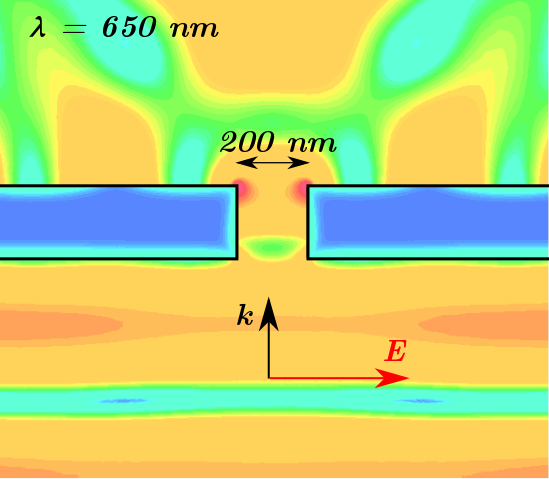
\includegraphics[scale=.3]{E_squared_final.png}
        \caption{Subwavelength Transmission through a Silver slit}
      \end{figure}
      \end{column}%
    \end{columns}
  \end{frame}
% ------------------------------------------------------------
% ------------------------------------------------------------
% ------------------------------------------------------------
% ------------------------------------------------------------
% ------------------------------------------------------------
% ------------------------------------------------------------
% ------------------------------------------------------------
% ------------------------------------------------------------
\begin{frame}
  \frametitle{Background}
  \framesubtitle{Optical Nanoantennas}

  \begin{columns} % align columns
    \begin{column}{.45\textwidth}
      % \begin{minipage}[T][.1\textheight][c]{\linewidth}
      \vspace*{-1cm}
      \begin{itemize}
        \item Convert Localized near-field to efficient far-field radiation
        \item Low Q-factor
        \item Extremely small size
        \item \color{red}{High Purcell Factor}
      \end{itemize}
      \begin{equation} \nonumber
        \mathrm{P}  = \frac{\mathrm{Q}}{\mathrm{V}}
      \end{equation}
      \begin{itemize}
        \item Directive radiation
      \end{itemize}
      % \end{minipage}
      %
    \end{column}
    %
    \begin{column}{.55\textwidth}
      \vspace*{-1cm}
      % Use this to preserve fonts from Inkspace
      \begin{figure}
        \hspace*{-1cm}
        \def\svgwidth{\linewidth}
        \input{figures/curto.pdf_tex}
        \caption{Optical resonant cavities for electric field enhancement}
      \end{figure}
      \end{column}%
    \end{columns}
  \end{frame}
% ------------------------------------------------------------
% ------------------------------------------------------------
% ------------------------------------------------------------
% ------------------------------------------------------------
% ------------------------------------------------------------
% ------------------------------------------------------------
% ------------------------------------------------------------
% ------------------------------------------------------------
\begin{frame}
  \frametitle{Background}
  \framesubtitle{Optical Nanoantennas (contd.)}

  \begin{columns} % align columns
    \begin{column}{.45\textwidth}
      \begin{minipage}[T][.1\textheight][c]{\linewidth}
        \begin{itemize}
          \item Scaled-down microwave designs
          \begin{itemize}
            \item[-] Directivity: Yagi-Uda antenna
            \item[-] Broadband: Bowtie antenna
          \end{itemize}
        \end{itemize}
        \begin{figure}
          \includegraphics[scale=.03]{bowtie_field_map.png}
          % \caption{Subwavelength Transmission through a Silver slit}
        \end{figure}
      \end{minipage}
    \end{column}
    %
    \begin{column}{.55\textwidth}
      % Use this to preserve fonts from Inkspace
      \hspace*{-1cm}
      \vspace*{-1cm}
      \begin{figure}
        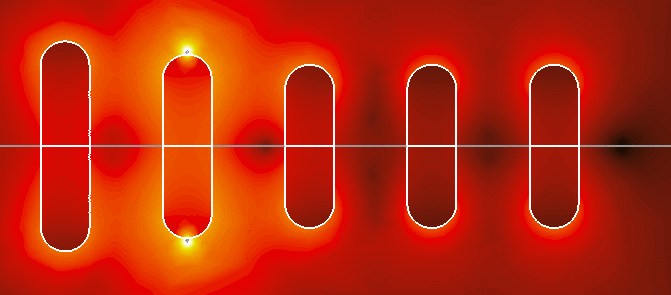
\includegraphics[scale=.04]{yagi_fields.png}
        % \caption{Subwavelength Transmission through a Silver slit}
      \end{figure}
      \hspace*{-1cm}
      \vspace*{-1.2cm}
      \begin{figure}

        \includegraphics[scale=.3]{yagi_patterna.png}
        % \caption{Subwavelength Transmission through a Silver slit}
      \end{figure}
      \end{column}%
    \end{columns}
  \end{frame}
  % ------------------------------------------------------------
  % ------------------------------------------------------------
  % ------------------------------------------------------------
  % ------------------------------------------------------------
  % ------------------------------------------------------------
  % ------------------------------------------------------------
  % ------------------------------------------------------------
  \begin{frame}
    \frametitle{Background}
    \framesubtitle{Optical Nanoantennas}
    \begin{columns}[T] % align columns
      \begin{column}{.5\textwidth}
        \begin{itemize}
          \item Metal-dielectric Interface
        \end{itemize}
        \begin{equation} \nonumber
          k_{sp}=\frac{\O}{c}\sqrt {\dfrac {\E_{1}\E_{2}(\O)} {\E_{1} + \E_{2}(\O)}}
          \label{eq:dis_spp}
        \end{equation}
        \begin{itemize}
          \item Accurate material description using Drude-critical points
        \end{itemize}
        \begin{equation} \nonumber
          \E_2(\O) = \E_{\inf} - \frac{\O_{d}^{2}}{\O^2 + j\gamma \O} + \sum \limits_{i = 1}^N G_i(\O)
          \label{eq:eps_drude_cp}
        \end{equation}
        \begin{equation} \nonumber
          G_i(\O) = C_i \left[ \frac{e^{j \phi_i}}{\O_i - \O - j \Gamma_i} + \frac{e^{-j \phi_i}}{\O_i + \O + j \Gamma_i} \right]
          \label{eq:CP_terms}
        \end{equation}
      \end{column}
      \begin{column}[T]{.5\textwidth}
        \centering
          \begin{figure}
            \vspace*{-2cm}
            \tikzset{
            font={\fontsize{18pt}{18}\selectfont}}
            \includegraphics[width = .75\linewidth]{figures/ep_silver.tikz}
            \label{fig:ep_silver}
          \end{figure}
          \begin{figure}
            \vspace*{-.3cm}
            \tikzset{
            font={\fontsize{18pt}{18}\selectfont}}
            \includegraphics[width = .75\linewidth]{figures/disp_silver.tikz}
            \label{fig:disp_silver}
          \end{figure}
        % \begin{figure}
        %   \vspace*{-2cm}
        %   \subfloat{\includegraphics[width = .75\linewidth]{figures/ep_silver.tikz}
        %   \label{fig:ep_gold}}
        %   \subfloat{\includegraphics[width = .75\linewidth]{figures/disp_silver.tikz}
        %   \label{fig:ep_silver}}
        % \end{figure}
      \end{column}
    \end{columns}
  \end{frame}
% ------------------------------------------------------------
% ------------------------------------------------------------
% ------------------------------------------------------------
% ------------------------------------------------------------
% ------------------------------------------------------------
% ------------------------------------------------------------
% ------------------------------------------------------------
% ------------------------------------------------------------
% ------------------------------------------------------------
% ------------------------------------------------------------
% ------------------------------------------------------------
% ------------------------------------------------------------
% ------------------------------------------------------------
% ------------------------------------------------------------
% ------------------------------------------------------------
% ------------------------------------------------------------

\begin{frame}[t]
  \frametitle{Nanoscale Imaging scheme}
  \framesubtitle{Basics}
  \begin{columns}[T] % align columns
    \begin{column}{.4\textwidth}
      \begin{outline}[itemize]
        \1 Structured Illumination
        \2 Periodic sine pattern
        \1 Moiré Fringes
        \2 Frequency modulation of two patterns
        \2 Resulting low-frequency signal
        \1 Linear scheme
        \2 Low light intensity
      \end{outline}
    \end{column}
    %%
    %%
    \begin{column}[T]{.6\textwidth}
      \begin{center}
        \begin{figure}[t!]
          \vspace*{-2cm}
          \centering
          \subfloat{\scalebox{.07}{\input{figures/fine_lines.pdf_tex}}
          \label{fig:test}} \hfil
          \subfloat{\scalebox{.07}{\input{figures/fine_lines_2.pdf_tex}}
          \label{fig:sim_hi}}
        \end{figure}
        \begin{figure}
          \vspace*{-.5cm}
          \centering
          \def\svgwidth{.6\linewidth}
          \input{figures/fine_lines_moire.pdf_tex}
        \end{figure}
      \end{center}
      \end{column}%
    \end{columns}
  \end{frame}
  % ------------------------------------------------------------
  % ------------------------------------------------------------
  % ------------------------------------------------------------
  % ------------------------------------------------------------
  % ------------------------------------------------------------
  % ------------------------------------------------------------
  % ------------------------------------------------------------
  % ------------------------------------------------------------
  % ------------------------------------------------------------
  % ------------------------------------------------------------
  % ------------------------------------------------------------
  % ------------------------------------------------------------
  % ------------------------------------------------------------
  % ------------------------------------------------------------
  \begin{frame}[t]
    \frametitle{Nanoscale Imaging scheme}
    \framesubtitle{Setup}
    \begin{center}
      \begin{figure}[t!]
        \centering \vspace*{-.5cm}
        {\scalebox{.55}{\input{figures/mstruc_gated.pdf_tex}}
        % \resizebox{5in}{!}{\input{figures/mstruc_gated.pdf_tex}}
        \label{fig:struct}}
      \end{figure}
    \end{center}
  \end{frame}

  % ------------------------------------------------------------
  % ------------------------------------------------------------
  % ------------------------------------------------------------
  % ------------------------------------------------------------
  % ------------------------------------------------------------
  % ------------------------------------------------------------
  % ------------------------------------------------------------
  % ------------------------------------------------------------
  % ------------------------------------------------------------
  % ------------------------------------------------------------
  % ------------------------------------------------------------
  % ------------------------------------------------------------
  % ------------------------------------------------------------
  % ------------------------------------------------------------
  \begin{frame}[t]
    \frametitle{Nanoscale Imaging scheme}
    \framesubtitle{Working Principle}
    \begin{outline}[itemize]
      \1 Illumination signal
    \end{outline}
    \begin{equation} \nonumber
      I(\v r) = 1 + \cos(\v k_{\p} \cdot \v r + \phi)
      \label{eq:intensity}
    \end{equation} \vspace*{-.5cm}
    \begin{outline}[itemize]
      \1 Observed Image (Spatial domain)
    \end{outline}
    \begin{equation} \nonumber
      M(\v r) = \left[ F(\v r) \cdot I(\v r) \right] \otimes H(\v r)
      \label{eq:m_spatial_image}
    \end{equation} \vspace*{-.5cm}
    \begin{outline}[itemize]
      \1 Fourier transformed Image
    \end{outline}
    \begin{equation} \nonumber
      \begin{split}
        \ti M(\v k) &= \left[ \ti F(\v k) \otimes \ti I(\v k) \right] \cdot \ti H(\v k) \\
        &= \frac{1}{2} \left[ 2\ti F(\v k) + \ti F(\v k - \v k_{\p}) \e^{- \j \phi} + \ti F(\v k + \v k_{\p}) \e^{\j \phi} \right] \cdot \ti H(\v k)
      \end{split}
      \label{eq:m_ft}
    \end{equation}
  \end{frame}
  % ------------------------------------------------------------
  % ------------------------------------------------------------
  % ------------------------------------------------------------
  % ------------------------------------------------------------
  % ------------------------------------------------------------
  % ------------------------------------------------------------
  % ------------------------------------------------------------
  % ------------------------------------------------------------
  % ------------------------------------------------------------
  % ------------------------------------------------------------
  % ------------------------------------------------------------
  % ------------------------------------------------------------
  % ------------------------------------------------------------
  % ------------------------------------------------------------
  \begin{frame}[t]
    \frametitle{Nanoscale Imaging scheme}
    \framesubtitle{Image Reconstruction}
    \begin{center}
      \begin{figure}[t!]
        \centering \vspace*{-.5cm}
        \def\svgwidth{.55\linewidth}
        \input{figures/psim.pdf_tex}
        \label{fig:sim}
      \end{figure}
    \end{center}
  \end{frame}
  % ------------------------------------------------------------
  % ------------------------------------------------------------
  % ------------------------------------------------------------
  % ------------------------------------------------------------
  % ------------------------------------------------------------
  % ------------------------------------------------------------
  % ------------------------------------------------------------
  % ------------------------------------------------------------
  % ------------------------------------------------------------
  % ------------------------------------------------------------
  % ------------------------------------------------------------
  % ------------------------------------------------------------
  % ------------------------------------------------------------
  % ------------------------------------------------------------
  \begin{frame}[t]
    \frametitle{Nanoscale Imaging scheme}
    \framesubtitle{Image Reconstruction}
    \begin{center}
      \begin{figure}[t!]
        \centering
        \vspace*{-1cm}
        \subfloat{\includegraphics[width=2.1in]{figures/shifted1.tikz}
        \label{fig:shift}}
        \subfloat{\includegraphics[width=2.0in]{tuning.tikz}
        \label{fig:s_waves}}
        \label{fig:simulation1}
      \end{figure}
    \end{center}
  \end{frame}
  % ------------------------------------------------------------
  % ------------------------------------------------------------
  % ------------------------------------------------------------
  % ------------------------------------------------------------
  % ------------------------------------------------------------
  % ------------------------------------------------------------
  % ------------------------------------------------------------
  % ------------------------------------------------------------
  % ------------------------------------------------------------
  % ------------------------------------------------------------
  % ------------------------------------------------------------
  % ------------------------------------------------------------
  % ------------------------------------------------------------
  % ------------------------------------------------------------
  \setcounter{subfigure}{0}% Reset subfigure/subfloat counter
  \begin{frame}[t]
    \frametitle{Nanoscale Imaging scheme}
    \framesubtitle{Results}
    \begin{figure}[!htbp] \vspace*{-1cm} \centering \hspace*{-.25cm}
      \subfloat[]{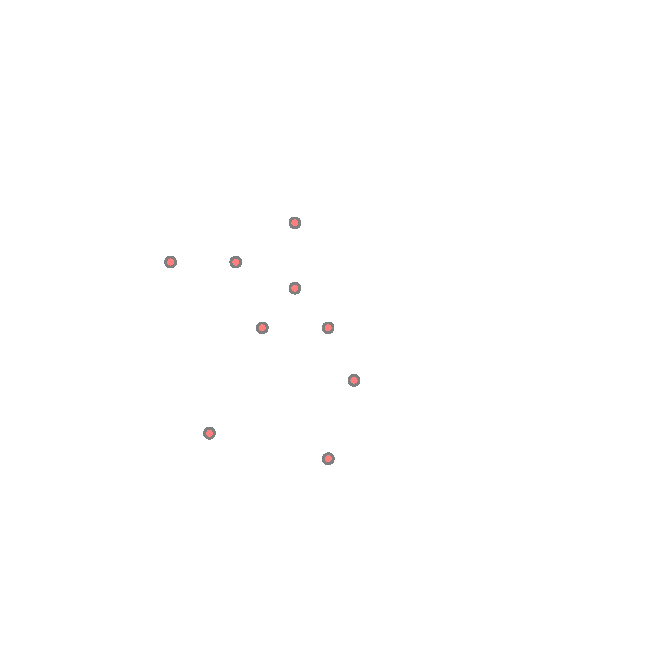
\includegraphics[height = 1.7in]{test_sample.tikz}
      \label{fig:test}}
      \subfloat[]{\includegraphics[height = 1.7in]{plsim_153.tikz}
      \label{fig:sim_lo}}
      \subfloat[]{\includegraphics[height = 1.7in]{plsim_75.tikz}
      \label{fig:sim_hi}}
      \caption{(a) Sample distribution. Simulation of the reconstructed sample image at: (b) $\Re k_{\p} = 39.5$ (c) $\Re k_{\p} = 80$}
      \label{fig:simulation}
    \end{figure}
  \end{frame}
  % ------------------------------------------------------------
  % ------------------------------------------------------------
  % ------------------------------------------------------------
  % ------------------------------------------------------------
  % ------------------------------------------------------------
  % ------------------------------------------------------------
  % ------------------------------------------------------------
  % ------------------------------------------------------------
  % ------------------------------------------------------------
  % ------------------------------------------------------------
  % ------------------------------------------------------------
  % ------------------------------------------------------------
  % ------------------------------------------------------------
  % ------------------------------------------------------------
  % ------------------------------------------------------------
  % ------------------------------------------------------------
  % ------------------------------------------------------------
  % ------------------------------------------------------------
  % ------------------------------------------------------------
  % ------------------------------------------------------------
  % ------------------------------------------------------------
  \section{Conclusion}
  \begin{frame}
    \frametitle{Summary}
    \framesubtitle{Two-dimensional plasmonic devices}
    \begin{itemize}
      \item Subwavelength wave phenomena at optical and terahertz frequencies
      \item Realization of terahertz sources and sensors
      \item 2D nature of waves permits subwavelength confinement
      \item Plasmonic activity
      \item Nanoscale imaging using terahertz plasma waves
    \end{itemize}
  \end{frame}
  % ------------------------------------------------------------
  % ------------------------------------------------------------
  % ------------------------------------------------------------
  % ------------------------------------------------------------
  % ------------------------------------------------------------
  % ------------------------------------------------------------
  % ------------------------------------------------------------
  \begin{frame}
    \frametitle{Acknowledgements}
    \framesubtitle{Sponsorship}
    \begin{itemize}
      \item The Fulbright Program
    \end{itemize}
    \begin{figure}
      \centering
      \def\svgwidth{.4\linewidth}
      \input{figures/fulbright.pdf_tex}
      % \caption{(a). Actual and its equivalent models for the (b) external and, (c) Internal region }
    \end{figure}
  \end{frame}
  % ------------------------------------------------------------
  % ------------------------------------------------------------
  % ------------------------------------------------------------
  % ------------------------------------------------------------
  % ------------------------------------------------------------
  % ------------------------------------------------------------
  % ------------------------------------------------------------
  \begin{frame}[plain,c]
    \begin{center}
      \Huge Thank you!
    \end{center}
  \end{frame}
  % ------------------------------------------------------------
  % ------------------------------------------------------------
  % ------------------------------------------------------------
  % ------------------------------------------------------------
  % ------------------------------------------------------------
  % ------------------------------------------------------------
  % ------------------------------------------------------------
  \begin{frame}[plain,c]
    \begin{center}
      \Huge Questions?
    \end{center}
  \end{frame}
  \end{document}
